\section*{Lagrangian Systems and the Principle of Least Action}
Mechanical systems, i.e. a pendulum, are modelled using the language of differential geometry. Thus it is necessary to introduce the relevant physical counterparts. 

\begin{definition}[Configuration Space]
	A \bld{configuration space}\index{Configuration space} is defined to be a finite-dimensional smooth manifold.
\end{definition}

\begin{definition}[Motion]
	A \bld{motion in a configuration space $M$}\index{Motion} is defined to be a path $\gamma \in C^\infty(J, M)$, where $J \subseteq \mathbb{R}$ is an interval.
\end{definition}

\begin{definition}[State]
	A \bld{state of the configuration space}\index{State} is defined to be an element of the tangent bundle of the configuration space, called the \bld{state space}\index{Space!state}.
\end{definition}

Also in classical mechanics, one has to rely on basic principles, which are to some extent experimentally verified. One of the most fundamental is the following.

\begin{axiom}[Newton-Laplace Determinacy Principle]
	\label{ax:NL_determinacy_principle}
	A motion in a configuration space is completely determined by a state at some instant.
\end{axiom}

The Newton-Laplace determinacy principle \ref{ax:NL_determinacy_principle} motivates our main definition of this chapter.

\begin{definition}[Lagrangian System]
	A \bld{Lagrangian system}\index{Lagrangian!system} is defined to be a tuple $(M,L)$ consisting of a smooth manifold $M$ and a function $L \in C^\infty(TM \times \mathbb{R})$, called a \bld{Lagrangian function}\index{Lagrangian!function}.
\end{definition}

\begin{example}
	\label{ex:Lagrangian}
	For a smooth manifold $M$ let $T \in C^\infty(TM \times \mathbb{R})$ and $V \in C^\infty(M \times \mathbb{R})$. Define $L \in C^\infty(TM \times \mathbb{R})$ by $L := T - V$. In this situation, $T$ is called the \bld{kinetic energy}\index{Energy!kinetic} and $V$ is called the \bld{potential energy}\index{Energy!potential}.
\end{example}

\begin{definition}[Path Space]
	\label{def:path_space}
	Let $M$ be a smooth manifold, $x_0,x_1 \in M$ and $t_0, t_1 \in \mathbb{R}$ with $t_0 \leq t_1$. Define the \bld{path space of $M$ connecting $(x_0,t_0)$ and $(x_1,t_1)$}\index{Space!path} to be the set
	\begin{equation}
		\label{eq:path_space}
		\mathcal{P}(M)^{x_0,t_0}_{x_1,t_1} := \cbr[0]{\gamma \in C^\infty(\intcc[0]{t_0,t_1},M) : \gamma(t_0) = x_0 \text{ and } \gamma(t_1) = x_1}.
	\end{equation}
\end{definition}

\begin{remark}
	For the sake of simplicity, we will just use the terminology \emph{path space} for $\mathcal{P}(M)^{x_0,t_0}_{x_1,t_1}$ and simply write $\mathcal{P}(M)$. We implicitely assume the conditions of definition \ref{def:path_space}, however.
\end{remark}

\begin{definition}[Variation]
	\label{def:variation}
	Let $\mathcal{P}(M)$ be a path space and $\gamma \in \mathcal{P}(M)$. A \bld{variation of $\gamma$}\index{Variation} is defined to be a morphism $\Gamma \in C^\infty(\intcc[0]{t_0,t_1} \times \intcc[0]{-\varepsilon_0,\varepsilon_0},M)$ for some $\varepsilon_0 > 0$ and such that
	\begin{itemize}[wide=0pt]
		\item $\Gamma(t,0) = \gamma$ for all $t \in \intcc[0]{t_1,t_0}$.
		\item $\Gamma(t_0,\varepsilon) = x_0$ for all $\varepsilon \in \intcc[0]{-\varepsilon_0,\varepsilon_0}$.
		\item $\Gamma(t_1,\varepsilon) = x_1$ for all $\varepsilon \in \intcc[0]{-\varepsilon_0,\varepsilon_0}$.
	\end{itemize}
\end{definition}

\begin{remark}
	If $\Gamma$ is a variation of $\gamma \in \mathcal{P}(M)$, we write $\gamma_\varepsilon(-) := \Gamma(-,\varepsilon)$ for all $\varepsilon \in \intcc[0]{-\varepsilon_0,\varepsilon_0}$.
\end{remark}

\begin{example}[Perturbation of a Path along a Single Direction]
	\label{ex:perturbation_along_single_direction}
	Let $M$ be a smooth manifold with $\dim M = n$, $(U,\varphi)$ a chart and suppose that $\gamma$ is a path in $U$. With respect to this chart, we can write the coordinate representation of $\gamma$ as
	\begin{equation*}
		\gamma(t) = \del[1]{\gamma^1(t),\dots,\gamma^n(t)}
	\end{equation*}
	\noindent for any $t \in \intcc[0]{t_0,t_1}$. Let $f \in C^\infty_c\intoo[0]{t_0,t_1}$. Consider the family $\Gamma : \intcc[0]{t_0,t_1} \times \intcc[0]{-\varepsilon_0,\varepsilon_0} \to M$ defined by
	\begin{equation*}
		\Gamma(t,\varepsilon) := (\iota \circ \varphi^{-1})\del[1]{\gamma^1(t),\dots,\gamma^i(t) + \varepsilon f(t),\dots,\gamma^n(t)}
	\end{equation*}
	\noindent where $\iota : U \hookrightarrow M$ denotes inclusion and $\varepsilon_0 > 0$ is to be determined. By exercise \ref{ex:U_delta_neighbourhood}, there exists $\delta > 0$ such that
	\begin{equation*}
		U_\delta := \cbr[0]{x \in \mathbb{R}^n : \dist(x,\gamma(\intcc[0]{t_0,t_1})) < \delta} \subseteq \varphi(U).
	\end{equation*}
	Choose $\varepsilon_0 > 0$ such that $0 < \varepsilon_0 < \delta/\norm{f}_\infty$. Then in coordinates
	\begin{equation*}
		\dist\del[1]{\gamma_\varepsilon(t), \gamma(\intcc[0]{t_0,t_1})} \leq \abs[0]{\gamma_\varepsilon(t) - \gamma(t)} = \abs{\varepsilon} \norm{f}_\infty \leq \varepsilon_0 \norm{f}_\infty < \delta 
	\end{equation*}
	\noindent for all $t \in \intcc[0]{t_0,t_1}$. Hence $\gamma_\varepsilon(t) \in U_\delta$ and thus $\gamma_\varepsilon(t) \in \varphi(U)$. Therefore, $\Gamma$ is indeed well-defined. Moreover, it is easy to show that the properties of definition \ref{def:variation} holds, therefore, $\Gamma$ is a variation of $\gamma$. In fact, this example shows, that any path $\gamma$ contained in a single chart admits infinitely many variations. An example of such a variation is shown in figure \ref{fig:variation}.

	\begin{figure}[h!tb]
		\centering
		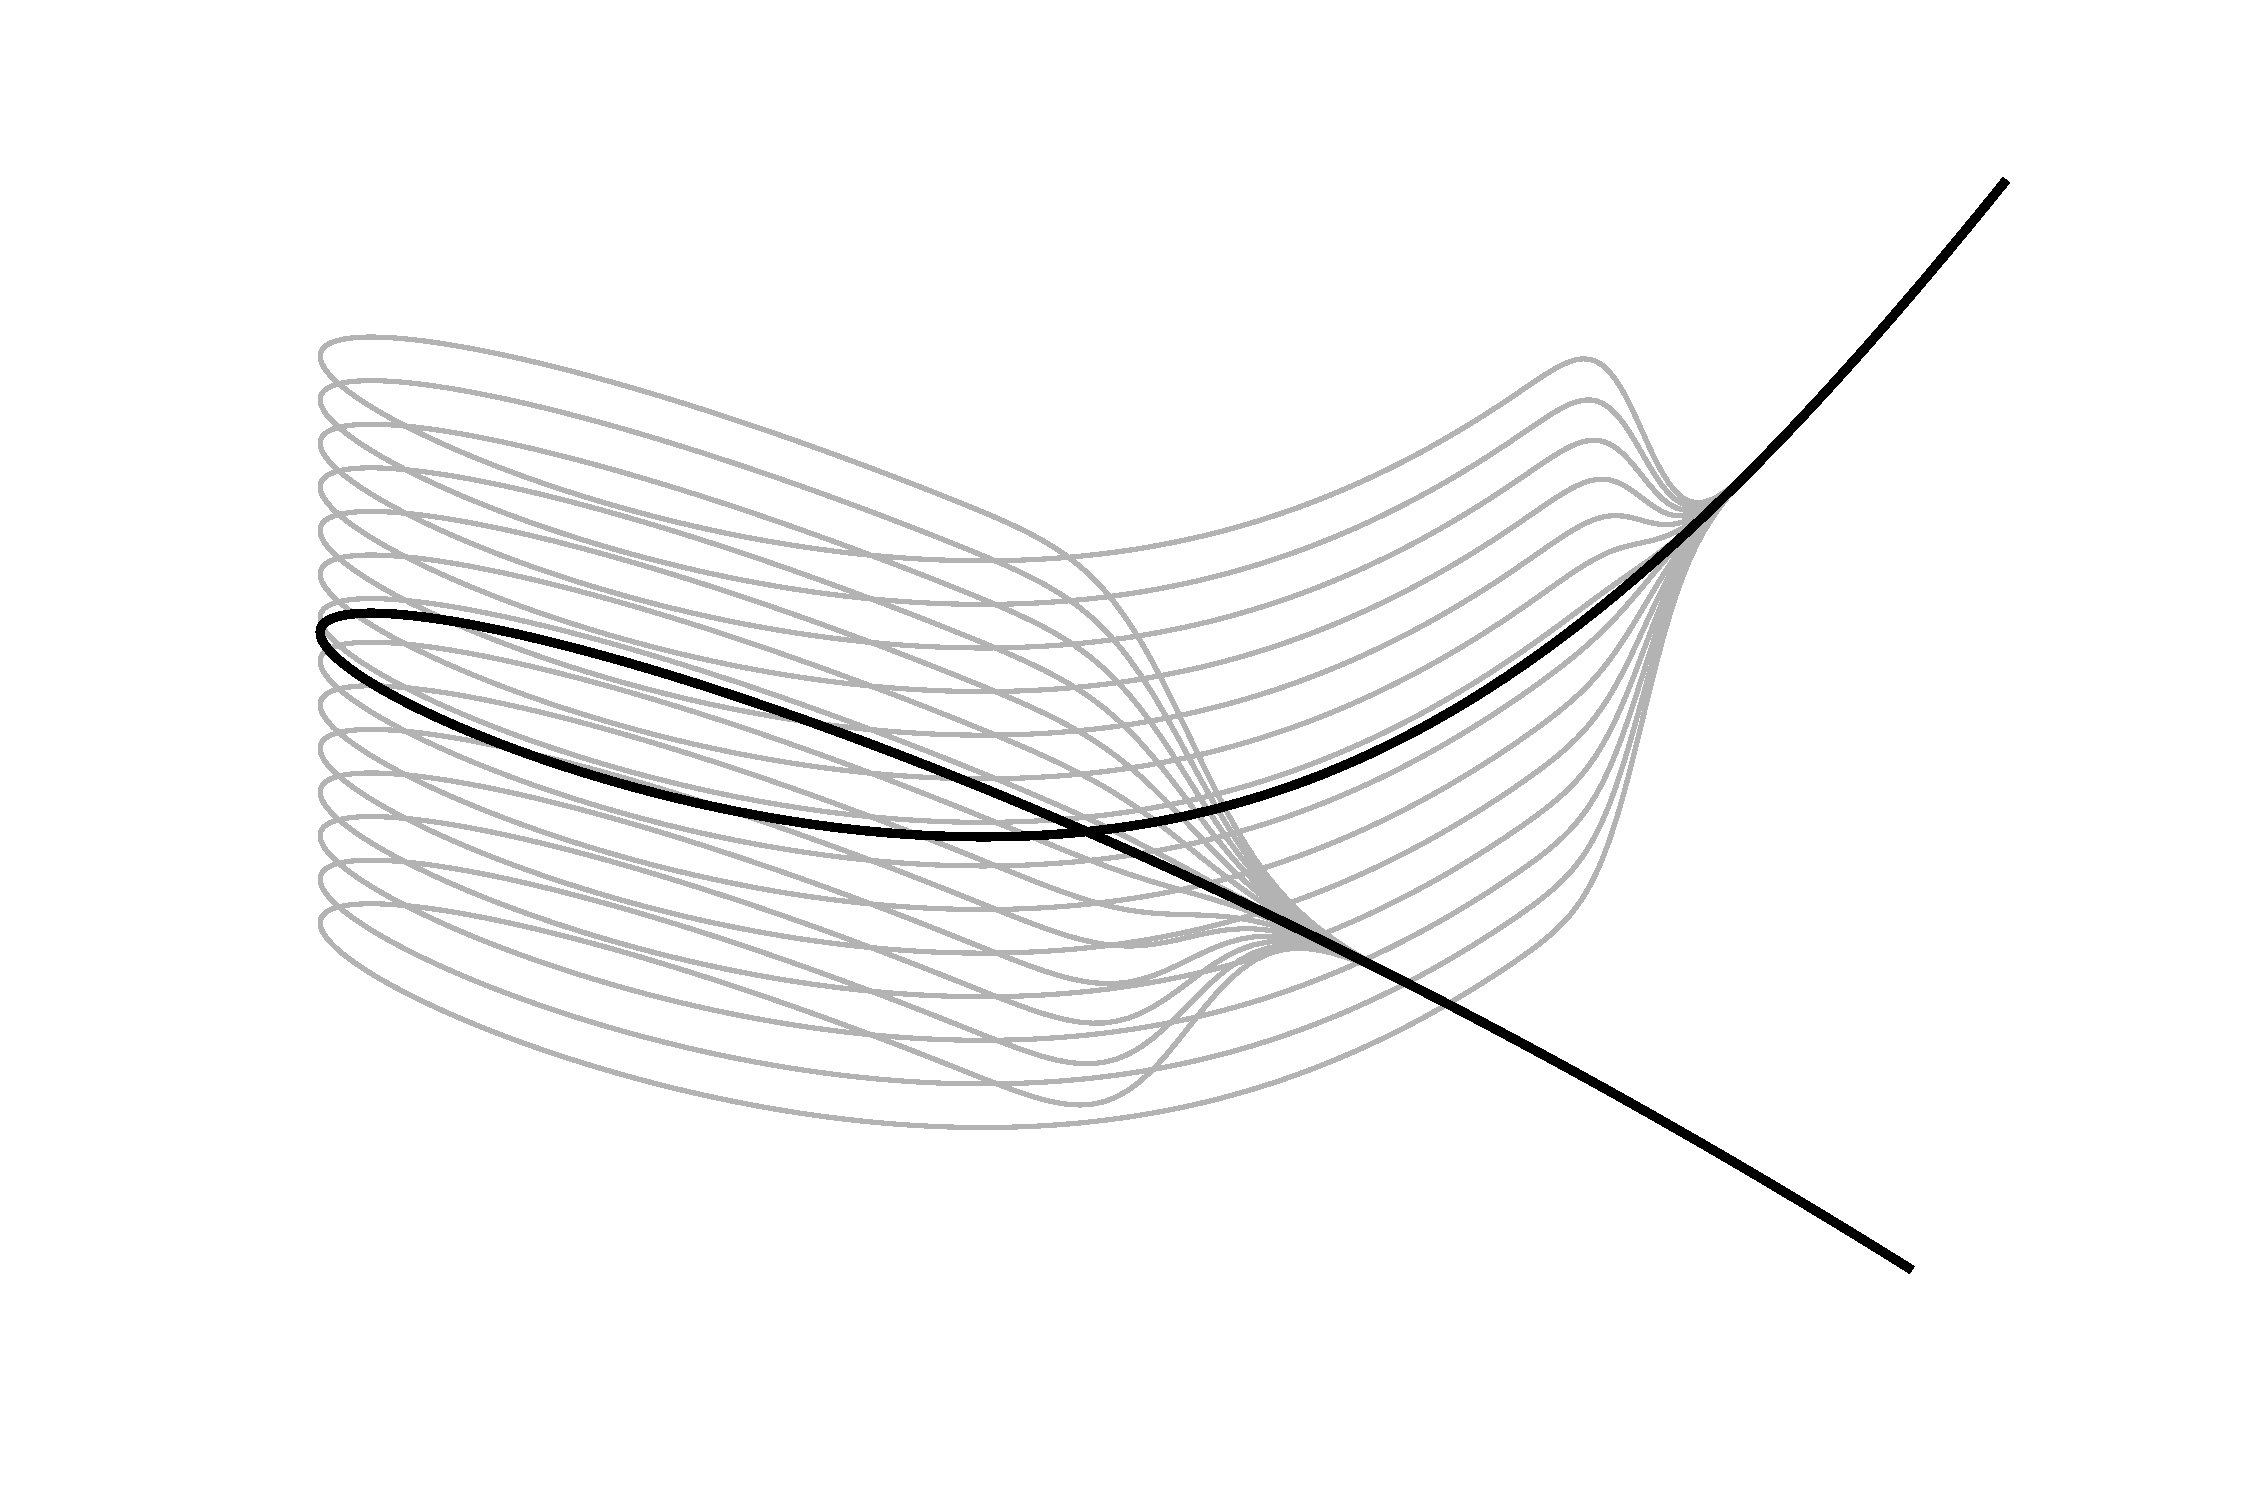
\includegraphics[width = .83\textwidth]{variation.pdf}
		\caption{Example of a variation of the path $\gamma(t) = (\gamma^1(t),\gamma^2(t))$ in $\mathbb{R}^2$ defined by $\gamma(t) := (t^2 + \sin(t)\cos(t),t^3 - t)$ for $t \in \intcc[0]{-\frac{3}{2},\frac{3}{2}}$ along the second coordinate using a smooth bump function as in \cite[42]{lee:smooth_manifolds:2013}.}
		\label{fig:variation}
	\end{figure}
\end{example}

\begin{exercise}
	\label{ex:U_delta_neighbourhood}
	Let $U \subseteq \mathbb{R}^n$ open and $A \subseteq U$ closed. Then there exists $\delta > 0$ such that
	\begin{equation*}
		U_\delta := \cbr[0]{x \in \mathbb{R}^n : \dist(x,A) < \delta} \subseteq U.
	\end{equation*}
\end{exercise}

\begin{definition}[Action Functional]
	Let $(M,L)$ be a Lagrangian system and $\mathcal{P}(M)$ be a path space. The morphism $S : \mathcal{P}(M) \to \mathbb{R}$ defined by
	\begin{equation*}
		S(\gamma) := \int_{t_0}^{t_1} L\del[0]{\gamma(t),\dot{\gamma}(t),t} dt
	\end{equation*}
	\noindent is called the \bld{action functional associated to the Lagrangian system $(M,L)$}\index{Action functional}.
\end{definition}

Motions of Lagrangian systems are characterized by an axiom.

\begin{axiom}[Hamilton's Principle of Least Action]\index{Hamilton!'s principle of least action}
	\label{ax:Hamilton_least_action}
	Let $(M,L)$ be a Lagrangian system and $\mathcal{P}(M)$ be a path space. A path $\gamma \in C^\infty(\intcc[0]{t_0,t_1},M)$ describes a motion of $(M,L)$ between $(x_0,t_0)$ and $(x_1,t_1)$ if and only if 
	\begin{equation}
		\frac{d}{d\varepsilon}\bigg\vert_{\varepsilon = 0} S(\gamma_\varepsilon) = 0
	\end{equation}
	\noindent for all variations $\gamma_\varepsilon$ of $\gamma$.
\end{axiom}

\begin{definition}[Extremal]
	A motion of a Lagrangian system between two points is called an \bld{extremal of the action functional $S$}\index{Extremal}.
\end{definition}

The Newton-Laplace determinacy principle \ref{ax:NL_determinacy_principle} implies that motions of mechanical systems can be described as solutions of second order ordinary differential equations. That this is indeed the case, is shown by the next theorem.

\begin{theorem}[Euler-Lagrange Equations]
	\label{thm:EL_equations}
	Let $(M,L)$ be a Lagrangian system. If a path $\gamma \in C^\infty(\intcc[0]{t_0,t_1},M)$ describes a motion of $(M,L)$ between $(x_0,t_0)$ and $(x_1,t_1)$ then for all charts $(U,x^i)$
	\begin{equation}
		\label{eq:EL_equations}
		\pd{L}{x}\del[1]{\gamma(t),\dot{\gamma}(t),t} - \frac{d}{dt} \pd{L}{v}\del[1]{\gamma(t),\dot{\gamma}(t),t} = 0
	\end{equation}
	\noindent holds, where $(x^i,v^i)$ denotes the standard coordinates on $TM$. The system of equations \textup{(}\ref{eq:EL_equations}\textup{)} is referred to as the \bld{Euler-Lagrange equations}\index{Equations!Euler-Lagrange}.
\end{theorem}

\begin{proof}
	By Hamilton's principle of least action \ref{ax:Hamilton_least_action}, we may assume that $\gamma$ is an extremal of the action functional $S$. The proof is divided into two steps.
	\begin{enumerate}[label = \textit{Step \arabic*:},wide=0pt]
		\item \textit{Suppose that $\gamma$ of $S$ is conatined in a chart domain $U$.} Let $t \in \intcc[0]{t_0,t_1}$ and abreviate $p := (\gamma(t),\dot{\gamma}(t),t)$ Using the formula for the derivative of a function along a curve \cite[283]{lee:smooth_manifolds:2013}, we compute
			\begin{align*}
				\frac{d}{d\varepsilon}\bigg\vert_{\varepsilon = 0} L\del[0]{\gamma_\varepsilon(t),\dot{\gamma}_\varepsilon(t),t} &= dL_p\del[3]{\frac{d}{d\varepsilon}\bigg\vert_{\varepsilon = 0}\gamma_\varepsilon(t),\frac{d}{d\varepsilon}\bigg\vert_{\varepsilon = 0}\dot{\gamma}_\varepsilon(t),0}\\
				&= dL_p\del[3]{\frac{d\gamma_\varepsilon^j(t)}{d\varepsilon}(0)\frac{\partial}{\partial x^j}\bigg\vert_{\gamma(t)},\frac{d\dot{\gamma}_\varepsilon^j(t)}{d\varepsilon}(0)\frac{\partial}{\partial v^j}\bigg\vert_{\dot{\gamma}(t)},0}.
			\end{align*}
			\noindent for all variations $\gamma_\varepsilon$ of $\gamma$ in $U$. Moreover
			\begin{equation*}
				dL_p = \frac{\partial L}{\partial x^i}(p) dx^i\vert_p + \frac{\partial L}{\partial v^i}(p) dv^i\vert_p + \frac{\partial L}{\partial t}(p)dt\vert_p.
			\end{equation*}
			Therefore
			\begin{align*}
				0 &= \frac{d}{d\varepsilon}\bigg\vert_{\varepsilon = 0} S(\gamma_\varepsilon)\\
				&= \int_{t_0}^{t_1} \frac{d}{d\varepsilon}\bigg\vert_{\varepsilon = 0} L\del[0]{\gamma_\varepsilon(t),\dot{\gamma}_\varepsilon(t),t} dt\\
				&= \int_{t_0}^{t_1} dL_p\del[3]{\frac{d\gamma_\varepsilon^j(t)}{d\varepsilon}(0)\frac{\partial}{\partial x^j}\bigg\vert_{\gamma(t)},\frac{d\dot{\gamma}_\varepsilon^j(t)}{d\varepsilon}(0)\frac{\partial}{\partial v^j}\bigg\vert_{\dot{\gamma}(t)},0}\\
				&= \int_{t_0}^{t_1} \frac{\partial L}{\partial x^i}(p)\frac{d\gamma_\varepsilon^i(t)}{d\varepsilon}(0)dt + \int_{t_0}^{t_1}\frac{\partial L}{\partial v^i}(p)\frac{d\dot{\gamma}_\varepsilon^i(t)}{d\varepsilon}(0)dt\\
				&= \int_{t_0}^{t_1} \frac{\partial L}{\partial x^i}(p)\frac{d\gamma_\varepsilon^i(t)}{d\varepsilon}(0)dt + \int_{t_0}^{t_1}\frac{\partial L}{\partial v^i}(p)\del[3]{\frac{d\gamma_\varepsilon^i(t)}{d\varepsilon}(0)}'dt\\
				&= \int_{t_0}^{t_1} \frac{\partial L}{\partial x^i}(p)\frac{d\gamma_\varepsilon^i(t)}{d\varepsilon}(0)dt + \frac{\partial L}{\partial v^i}(p)\frac{d\gamma_\varepsilon^i(t)}{d\varepsilon}(0)\bigg\vert_{t_0}^{t_1} - \int_{t_0}^{t_1} \frac{d}{dt}\frac{\partial L}{\partial v^i}(p)\frac{d\gamma_\varepsilon^i(t)}{d\varepsilon}(0)dt\\
				&= \int_{t_0}^{t_1} \del[3]{\frac{\partial L}{\partial x^i}(p) - \frac{d}{dt}\frac{\partial L}{\partial v^i}(p)}\frac{d\gamma_\varepsilon^i(t)}{d\varepsilon}(0)dt 
			\end{align*}
			\noindent since $\gamma^i_\varepsilon(t_0)$ and $\gamma^i_\varepsilon(t_1)$ are constant by definition of a variation. Let $f \in C^\infty_c\intoo[0]{t_0,t_1}$, $j = 1,\dots,n$ and $\gamma_\varepsilon$ be the variation of $\gamma$ defined in example \ref{ex:perturbation_along_single_direction} along the $j$-th direction. Above computation therefore yields
			\begin{equation*}
				0 = \int_{t_0}^{t_1} \del[3]{\frac{\partial L}{\partial x^j}(p) - \frac{d}{dt}\frac{\partial L}{\partial v^j}(p)}f(t) dt
			\end{equation*}
			\noindent for all $f \in C^\infty_c\intoo[0]{t_0,t_1}$. Hence the fundamental lemma of calculus of variations \ref{lem:fundamental_lemma} implies
			\begin{equation*}
				\frac{\partial L}{\partial x^j}(p) - \frac{d}{dt}\frac{\partial L}{\partial v^j}(p) = 0
			\end{equation*}
			\noindent for all $j = 1,\dots,n$.
		\item \textit{Suppose that $\gamma$ is an arbitrary extremal of $S$.} The key technical result used here is the following lemma.
			\begin{lemma}[Lebesgue Number Lemma]
				\label{lem:Lebesgue_number_lemma}
				Every open cover of a compact metric space admits a Lebesgue number, i.e. a number $\delta > 0$ such that every subset of the metric space with diameter less than $\delta$ is contained in a member of the family.
			\end{lemma}

			\begin{proof}
				See \cite[194]{lee:topological_manifolds:2011}.
			\end{proof}

			Let $(U_\alpha)_{\alpha \in A}$ be the smooth structure on $M$, i.e. the maximal smooth atlas. Since $\gamma$ is continuous, $\del[1]{\gamma^{-1}(U_\alpha)}_{\alpha \in A}$ is an open cover for $\intcc[0]{t_0,t_1}$. By the Lebesgue number lemma \ref{lem:Lebesgue_number_lemma}, this open cover admits a Lebesgue number $\delta > 0$. Let $k \in \mathbb{N}$ such that $(t_1 - t_0)/k < \delta$ and define
			\begin{equation*}
				t_i := \frac{i}{k}(t_1 - t_0) + t_0
			\end{equation*}
			\noindent for all $i = 0,\dots,k$. Then for all $i = 1,\dots,k$, $\gamma\vert_{\intcc[0]{x_{i - 1},x_i}}$ is contained in $U_\alpha$ for some $\alpha \in A$. Hence applying step $1$ yields the result.
	\end{enumerate}
\end{proof}

\begin{remark}
	\label{rem:global_chart}
	If a configuration space can be covered by a single chart, then the statement of theorem \ref{thm:EL_equations} becomes an equivalence.
\end{remark}

Due to the Newton-Laplace Determinacy Principle \ref{ax:NL_determinacy_principle}, the motions on a Lagrangian system are inherently characterized by the Lagrangian function and locally by the Euler-Lagrange equations (\ref{eq:EL_equations}). Hence any motion satisfies locally a system of second order ordinary differential equations. This system bears its own name.

\begin{definition}[Equations of Motion]
	The Euler-Lagrange equations \textup{(}\ref{eq:EL_equations}\textup{)} of a Lagrangian system are called the \bld{equations of motion}\index{Equations!of motion}.
\end{definition}

\begin{example}[Motions on Riemannian Manifolds]
	\label{ex:motions_on_Riemannian_manifolds}
	Let $(M,g)$ be a Riemannian manifold with $\dim M = n$ and consider the Lagrangian $L$ on $M$ defined in example \ref{ex:Lagrangian} with kinetic energy
	\begin{equation*}
		T(x,v,t) := \frac{1}{2}g_x(v,v) = \frac{1}{2}\abs{v}^2_g
	\end{equation*}
	\noindent and potential energy $V(x,t) := 0$ for $x \in M$, $v \in T_xM$ and $t \in \mathbb{R}$. Let $(U,x^i)$ be a chart on $M$. We compute
	\begin{align*}
		L(x,v,t) &= \frac{1}{2}g_{x}\del[0]{v,v}\\
		&= \frac{1}{2}g_{x}\del[3]{v^i\frac{\partial}{\partial x^i}\bigg\vert_x,v^j(t)\frac{\partial}{\partial x^j}\bigg\vert_x}\\
		&= \frac{1}{2}g_{x}\del[3]{\frac{\partial}{\partial x^i}\bigg\vert_x,\frac{\partial}{\partial x^j}\bigg\vert_x}v^iv^j\\
		&= \frac{1}{2}g_{ij}(x)v^iv^j,
	\end{align*}
	\noindent where $g_{ij}(x) := g_{x}\del[1]{\frac{\partial}{\partial x^i}\big\vert_x,\frac{\partial}{\partial x^j}\big\vert_x}$. Thus 
	\begin{equation*}
		\frac{\partial L}{\partial x^l}(x,v,t) = \frac{1}{2}\frac{\partial g_{ij}}{\partial x^l}(x)v^i v^j
	\end{equation*}
	\noindent and in particular
	\begin{equation*}
		\frac{\partial L}{\partial x^l}\del[1]{\gamma(t),\dot{\gamma}(t),t} = \frac{1}{2}\frac{\partial g_{ij}}{\partial x^l}\del[1]{\gamma(t)}\dot{\gamma}^i(t) \dot{\gamma}^j(t),
	\end{equation*}
	\noindent for all $l = 1,\dots,n$. Moreover
	\begin{equation*}
		\frac{\partial L}{\partial v^l}(x,v,t) = \frac{1}{2}g_{ij}(x)\delta^i_lv^j + \frac{1}{2}g_{ij}(x)v^i\delta^j_l = \frac{1}{2}g_{lj}(x)v^j + \frac{1}{2}g_{il}(x)v^i
	\end{equation*}
	\noindent implies
	\begin{align*}
		\frac{d}{dt}\frac{\partial L}{\partial v^l}\del[1]{\gamma(t),\dot{\gamma}(t),t} &= \frac{1}{2}\frac{d}{dt}g_{lj}(\gamma)\dot{\gamma}^j + \frac{1}{2}g_{lj}(\gamma)\ddot{\gamma}^j + \frac{1}{2}\frac{d}{dt}g_{il}(\gamma)\dot{\gamma}^i + \frac{1}{2}g_{il}(\gamma)\ddot{\gamma}^i\\
		&= \frac{1}{2}dg_{lj}(\dot{\gamma})\dot{\gamma}^j + \frac{1}{2}g_{lj}(\gamma)\ddot{\gamma}^j + \frac{1}{2}dg_{il}(\dot{\gamma})\dot{\gamma}^i + \frac{1}{2}g_{il}(\gamma)\ddot{\gamma}^i\\
		&= \frac{1}{2}\frac{\partial g_{lj}}{\partial x^k}\dot{\gamma}^k\dot{\gamma}^j + \frac{1}{2}g_{lj}(\gamma)\ddot{\gamma}^j + \frac{1}{2}\frac{\partial g_{il}}{\partial x^k}\dot{\gamma}^k\dot{\gamma}^i + \frac{1}{2}g_{il}(\gamma)\ddot{\gamma}^i\\
		&= \frac{1}{2}\frac{\partial g_{jl}}{\partial x^k}\dot{\gamma}^k\dot{\gamma}^j + \frac{1}{2}g_{jl}(\gamma)\ddot{\gamma}^j + \frac{1}{2}\frac{\partial g_{il}}{\partial x^k}\dot{\gamma}^k\dot{\gamma}^i + \frac{1}{2}g_{il}(\gamma)\ddot{\gamma}^i\\
		&= g_{il}\ddot{\gamma}^i + \frac{1}{2}\frac{\partial g_{jl}}{\partial x^i}\dot{\gamma}^i\dot{\gamma}^j + \frac{1}{2}\frac{\partial g_{il}}{\partial x^j}\dot{\gamma}^i\dot{\gamma}^j.
	\end{align*}
	Therefore the Euler-Lagrange equations (\ref{eq:EL_equations}) read
	\begin{equation*}
		0 = \frac{d}{dt}\frac{\partial L}{\partial v^l} - \frac{\partial L}{\partial x^l} = g_{il}\ddot{\gamma}^i + \frac{1}{2}\del[3]{\frac{\partial g_{jl}}{\partial x^i} + \frac{\partial g_{il}}{\partial x^j} - \frac{\partial g_{ij}}{\partial x^l}}\dot{\gamma}^i\dot{\gamma}^j,	
	\end{equation*}
	\noindent for all $l = 1,\dots,n$. Multiplying both sides by $g^{kl}$ yields
	\begin{equation}
		\label{eq:geodesic_equation}
		\ddot{\gamma}^k + \Gamma^k_{ij}\dot{\gamma}^i \dot{\gamma}^j = 0,
	\end{equation}
	\noindent for all $k = 1,\dots,n$, where
	\begin{equation*}
		\Gamma^k_{ij} := \frac{1}{2}g^{kl}\del[3]{\frac{\partial g_{jl}}{\partial x^i} + \frac{\partial g_{il}}{\partial x^j} - \frac{\partial g_{ij}}{\partial x^l}}
	\end{equation*}
	\noindent are the \bld{Christoffel symbols}\index{Symbols!Christoffel} with respect to the choosen chart (see \cite[70]{lee:Riemannian_manifolds:1997}). Equation (\ref{eq:geodesic_equation}) is called the \bld{geodesic equation}\index{Equations!geodesic} (see \cite[58]{lee:Riemannian_manifolds:1997}). Hence extremals $\gamma$ of the action functional satisfy the geodesic equation and are therefore geodesics on the Riemannian manifold $M$.
\end{example}

\begin{lemma}
	\label{lem:same_equations_of_motion}
	Let $(M,L)$ be a Lagrangian system and define $L + df \in C^\infty(TM \times \mathbb{R})$ by
	\begin{equation*}
		(L + df)(x,v,t) := L(x,v,t) + df_x(v)
	\end{equation*}
	\noindent for any $f \in C^\infty(M)$. Then $(M,L)$ and $(M,L + df)$ admit the same equations of motion.
\end{lemma}

\begin{proof}
	Let us denote the action function corresponding to $L + df$ by $\wtilde{S}$ and suppose $\gamma_\varepsilon$ is a variation of $\gamma$ in $M$. Using the formula for the derivative of a function along a curve \cite[283]{lee:smooth_manifolds:2013} we compute
	\begin{align*}
		\wtilde{S}(\gamma_\varepsilon) &= \int_{t_0}^{t_1}L(\gamma_\varepsilon(t),\dot{\gamma}_\varepsilon(t),t)dt + \int_{t_0}^{t_1}df_{\gamma_\varepsilon(t)}\del[1]{\dot{\gamma}_\varepsilon(t)}dt\\
		&= S(\gamma_\varepsilon) + \int_{t_0}^{t_1}(f \circ \gamma_\varepsilon)'(t)dt\\
		&= S(\gamma_\varepsilon) + f\del[1]{\gamma_\varepsilon(t_1)} - f\del[1]{\gamma_{\varepsilon}(t_0)}\\
		&= S(\gamma_\varepsilon) + f(x_1) - f(x_0).
	\end{align*}
	In particular
	\begin{equation*}
		\frac{d}{d\varepsilon}\bigg\vert_{\varepsilon = 0}\wtilde{S}(\gamma_\varepsilon) = \frac{d}{d\varepsilon}\bigg\vert_{\varepsilon = 0}S(\gamma_\varepsilon).
	\end{equation*}
\end{proof}

\begin{remark}
	Lemma \ref{lem:same_equations_of_motion} implies, that the Lagrangian of a mechanical system can only be determined up to differentials of smooth functions. Actually, in coordinates, also up to total time derivatives. Hence a \emph{law of motion}, that is a Lagrangian describing a certain mechanical system, is in fact an equivalence class of Lagrangian functions.
\end{remark}
